
\clearpage
\section{La liste d'adresses}
\label{bkm:Ref443738751}
Dans la liste d'adresses, toutes les personnes (utilisateurs) et entreprises (unités d'organisation) recensées dans CUBE PA sont affichées. Avec la fonction de filtre, les saisies recherchées peuvent être rapidement repérées.

\vspace{\baselineskip}

Les caractéristiques suivantes sont à prendre en compte lors de l'utilisation de la liste d'adresses :

% \liststyleWWviiiNumxiii
\begin{itemize}
\item
Un utilisateur de CUBE PA ayant les droits nécessaires peut ajouter de nouvelles personnes et unités d'organisation à la liste d'adresses ou modifier des saisies existantes.

\item
Les personnes qui ont été ajoutées de cette manière sont automatiquement disponibles dans tous les champs de sélection de personnes (par exemple affaires en suspens). Par contre, ces personnes nouvellement ajoutées ne peuvent pas se connecter à CUBE PA. Si ceci est désiré, l'administrateur peut aider, ou il faut prendre contact avec le support CUBE PA (voir chapitre \ref{bkm:Ref443502661}).

\item
Si une personne est attribuée à une entreprise, l'adresse de l'entreprise apparaît automatiquement dans la liste d'adresses. Si ceci n'est pas souhaité, par exemple à cause de différents lieux d'implantation de l'entreprise, une adresse spécifique peut être saisie pour la personne.

\item
Pour les utilisateurs qui sont activés et qui peuvent se connecter à CUBE PA, l'appartenance à une entreprise ne peut être modifiée que par l'administrateur pour des raisons de sécurité (droits d'accès). Avertissez l'administrateur ou le support CUBE PA Support si de telles mutations se produisent (voir chapitre \ref{bkm:Ref443502661}).

\item
Les saisies d'entreprises effectuées dans la liste d'adresses ne sont pas automatiquement disponibles comme soumissionnaires ou clients dans la fonction d'acquisition. Ceci doit être configuré en conséquence par l'administrateur.
\end{itemize}

\pagebreak
\subsection{Trouver des personnes ou des entreprises dans la liste d'adresses}

\begin{wrapfigure}[2]{l}{6.5cm}   % [x] Wie manche Zeile soll sich um die Grafik "brechen"
  \vspace{-35pt}      % Grundwert war 20; mit 30 schön oben beim Text ausgerichtet
  \begin{center}
    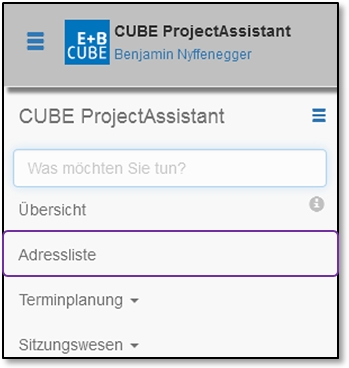
\includegraphics[width=1\linewidth]{../chapters/03_Adressliste/pictures/3-1_Menu_Adressliste.jpg}
  \end{center}
  \vspace{-20pt}
  \caption{Utiliser la liste d'adresses}
  \vspace{-10pt}
\end{wrapfigure}

Choisissez l'élément 'Liste d'adresses' du menu principal à gauche.

\vspace{7cm}

Une liste qui contient les adresses de toutes les personnes et entreprises enregistrées dans CUBE PA s'affiche :

\begin{figure}[H]
\center{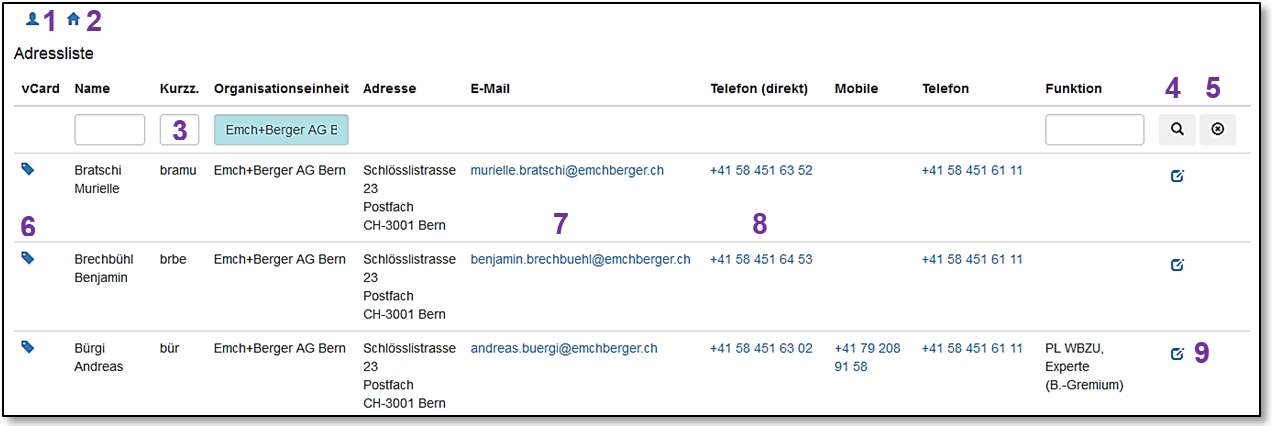
\includegraphics[width=1\linewidth]{../chapters/03_Adressliste/pictures/3-1_Adressliste_Uebersicht.jpg}}
\caption{Aperçu de la liste d'adresses}
% \label{fig:speciation}
\end{figure}

En haut à gauche vous pouvez ajouter de nouvelles personnes 
\includegraphics[height=12pt]{/Icons/Person.jpg} ou denouvelles entreprises 
\includegraphics[height=12pt]{/Icons/Haus.jpg}. Prenez en compte les caractéristiques qui ont été citées au début de ce chapitre (Chapitre \ref{bkm:Ref443738751}). \newline
Pour la recherche / le filtrage des enregistrements vous avez deux champs à disposition. Saisissez un mot-clé dans le champ 'Nom' et/ou 'Unité d'organisation' \col{(3)} et cliquez sur la loupe 
\includegraphics[height=12pt]{/Icons/Lupe_kl.jpg} \col{(4)} ou confirmez avec la touche Entrée. Toutes les saisies qui correspondent aux critères de recherche sont affichées. En cliquant sur la petite croix \col{(5)} vous pouvez effacer les critères de recherche. \newline
Vous avez la possibilité de télécharger une vCard (carte de visite par exemple pour Outlook). Cliquez sur le symbole vCard 
\includegraphics[height=12pt]{/Icons/vCard.jpg} \col{6)}. Vous aurez le choix de soit ouvrir ou sauvegarder la vCard .\newline
Cliquez sur l'adresse électronique \col{(7)} pour écrire un e-mail à la personne choisie. Cliquez sur le numéro de téléphone \col{(8)} pour appeler la personne par exemple par Skype (selon l'installation).\newline
Si vous cliquez sur le symbole de modification 
\includegraphics[height=12pt]{/Icons/Bearbeiten.jpg} \col{(9)}, vous pouvez changer les données d'une personne ou d'une entreprise. Pour ce faire vous devez disposer des droits d'accès nécessaires.

\subsection{Ajouter de nouvelles personnes ou entreprises dans la liste d'adresses}
Les utilisateurs autorisés peuvent ajouter de nouvelles personnes ou entreprises dans la liste d'adresses ou modifier des saisies existantes :

\vspace{\baselineskip}

\begin{tabular}{cc} %{cl}
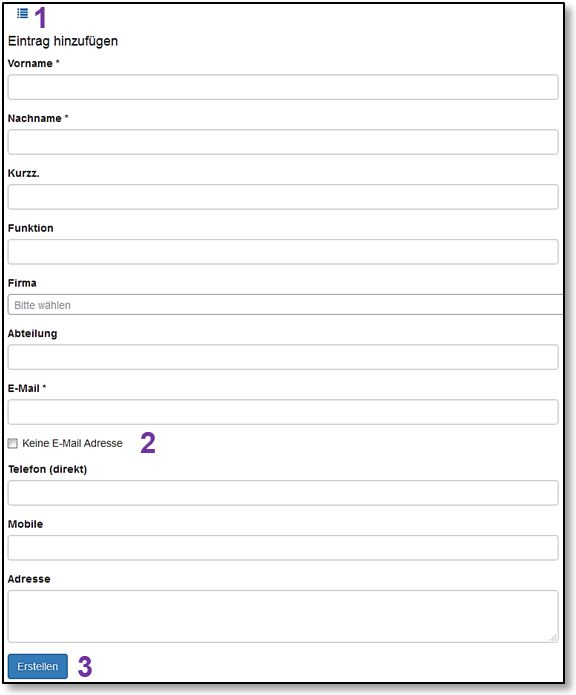
\includegraphics[width=0.49\textwidth]{32_Personeneintraege.jpg} & 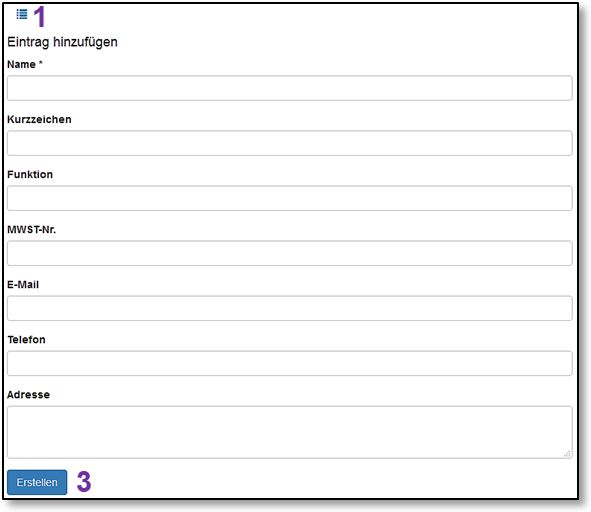
\includegraphics[width=0.49\textwidth]{32_Firmeneintraege.jpg} \\
Saisies de personnes & Saisie d'entreprises\\
\end{tabular}

% \begin{figure} 
%      \subfigure{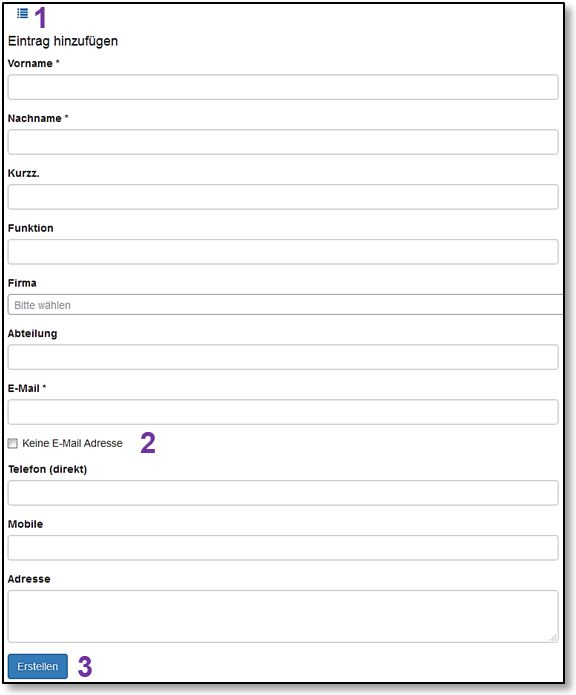
\includegraphics[width=0.49\textwidth]{32_Personeneintraege.jpg}} 
%      \subfigure{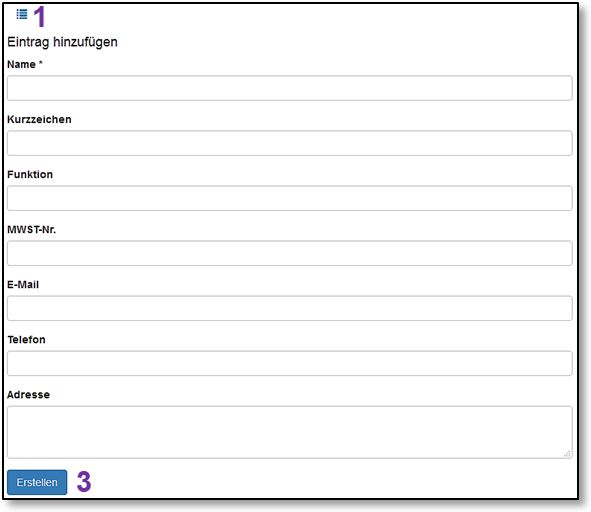
\includegraphics[width=0.49\textwidth]{32_Firmeneintraege.jpg}} 
% \caption{Die verschiedenen Eingabemasken der Adressliste} 
% \end{figure}

\vspace{\baselineskip}
Tous les champs marqués avec * sont des champs obligatoires qui doivent être remplis. Si une adresse électronique ne peut ou ne doit pas être saisie, ce champ obligatoire peut être contourné et laissé vide en cochant la case 'Pas d'adresse e-mail' \col{(2)}. Après avoir rempli les champs désirés/connus, la saisie peut être sauvegardée avec le bouton 'Créer' \col{(3)} et est à disposition dans la liste d'adresses. En cliquant sur le symbole de modification d'une donnée existante 
\includegraphics[height=12pt]{/Icons/Bearbeiten.jpg}, le même masque (voir plus haut) s'affiche. Toutes les données qui ont déjà été saisies se trouvent dans les champs correspondants et peuvent être modifiées. Comme mentionné au début du chapitre, seul l'administrateur peut changer l'appartenance d'une personne à une entreprise, pour des raisons de sécurité (droits d'accès).\newline
En cliquant sur le symbole de liste 
\includegraphics[height=12pt]{/Icons/Listensymbol_zurueck.jpg} \col{(1)} vous retournez à la liste d'adresses.
